
\subsection*{1.}

\begin{center}
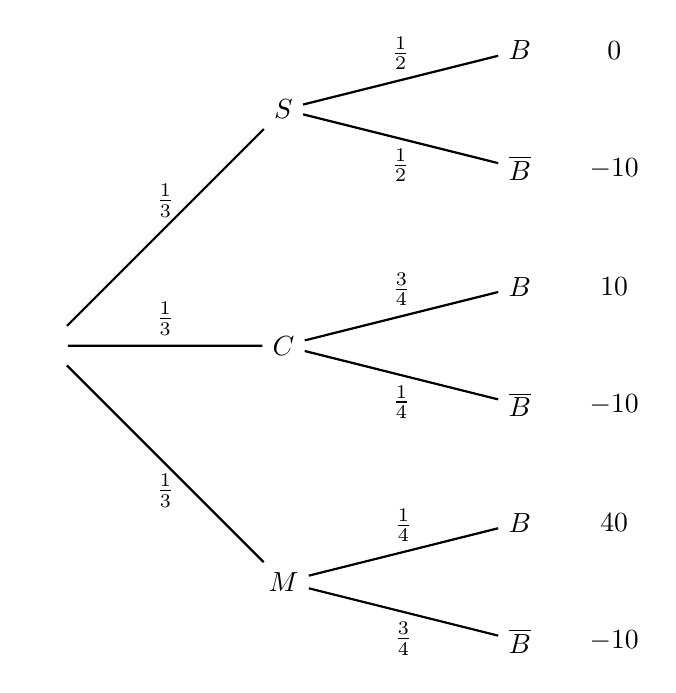
\begin{tikzpicture}[thick, scale=1.5]
\node (P_-1_0) at (-2,-2.5) {$\phantom{A}$};
\node (P_0_0) at (0,-0.5) {$S$};
\draw (P_-1_0) -- (P_0_0) node[midway, above] {$\frac13$};
\node (P_1_0) at (2,-0) {$B$};
\draw (P_0_0) -- (P_1_0) node[midway, above] {$\frac12$};
\node (P_2_0) at (2.8,-0) {$0$};
%\draw (P_1_0) -- (P_2_0) node[midway, above] {$$};
\node (P_1_1) at (2,-1) {$\overline{B}$};
\draw (P_0_0) -- (P_1_1) node[midway, below] {$\frac12$};
\node (P_2_1) at (2.8,-1) {$-10$};
%\draw (P_1_1) -- (P_2_1) node[midway, above] {$$};
\node (P_0_2) at (0,-2.5) {$C$};
\draw (P_-1_0) -- (P_0_2) node[midway, above] {$\frac13$};
\node (P_1_2) at (2,-2) {$B$};
\draw (P_0_2) -- (P_1_2) node[midway, above] {$\frac34$};
\node (P_2_2) at (2.8,-2) {$10$};
%\draw (P_1_2) -- (P_2_2) node[midway, above] {$$};
\node (P_1_3) at (2,-3) {$\overline{B}$};
\draw (P_0_2) -- (P_1_3) node[midway, below] {$\frac14$};
\node (P_2_3) at (2.8,-3) {$-10$};
%\draw (P_1_3) -- (P_2_3) node[midway, above] {$$};
\node (P_0_4) at (0,-4.5) {$M$};
\draw (P_-1_0) -- (P_0_4) node[midway, below] {$\frac13$};
\node (P_1_4) at (2,-4) {$B$};
\draw (P_0_4) -- (P_1_4) node[midway, above] {$\frac14$};
\node (P_2_4) at (2.8,-4) {$40$};
%\draw (P_1_4) -- (P_2_4) node[midway, above] {$$};
\node (P_1_5) at (2,-5) {$\overline{B}$};
\draw (P_0_4) -- (P_1_5) node[midway, below] {$\frac34$};
\node (P_2_5) at (2.8,-5) {$-10$};
%\draw (P_1_5) -- (P_2_5) node[midway, above] {$$};
\end{tikzpicture}
\end{center}

\subsection*{2.}

D'après la loi des probabilités totales :
\[
P(B) = P(S \cap B) + P(C \cap B) + P(M \cap B),
\]
ce qui donne :
\[
P(B) = P(S) \times P_S(B) + P(C) \times P_C(B) + P(M) \times P_M(B),
\]
\[
P(B) = \dfrac{1}{3} \times \dfrac{1}{2} + \dfrac{1}{3} \times \dfrac{3}{4} + \dfrac{1}{3} \times \dfrac{1}{4} = \dfrac{1}{6} + \dfrac{3}{12} + \dfrac{1}{12} = \dfrac{6}{12} = \dfrac{1}{2}.
\]

\subsection*{3.}

On a :
\[
P(X = 40) = P(M \cap B) = P(M) \times P_M(B) = \dfrac{1}{3} \times \dfrac{1}{4} = \dfrac{1}{12}.
\]

\subsection*{4.}

On a :
\begin{itemize}
    \item
    \(P(X = -10) = P(\overline{B}) = P(S \cap \overline{B}) + P(C \cap \overline{B}) + P(M \cap \overline{B})\),

\(P(X = -10) = \dfrac{1}{3} \times \dfrac{1}{2} + \dfrac{1}{3} \times \dfrac{1}{4} + \dfrac{1}{3} \times \dfrac{3}{4} = \dfrac{1}{6} + \dfrac{1}{12} + \dfrac{3}{12} = \dfrac{1}{2}\).
    \item \(P(X = 0) = P(S \cap B) = \dfrac{1}{3} \times \dfrac{1}{2} = \dfrac{1}{6}\).
    \item \(P(X = 10) = P(C \cap B) = \dfrac{1}{3} \times \dfrac{3}{4} = \dfrac{1}{4}\).
    \item \(P(X = 40) = P(M \cap B) = \dfrac{1}{3} \times \dfrac{1}{4} = \dfrac{1}{12}\).
\end{itemize}

D'où le tableau de la loi de probabilités :

\[
\begin{array}{|c|c|c|c|c|}
\hline
X & -10 & 0 & 10 & 40 \\
\hline
P(X = x_i) & \dfrac{1}{2} & \dfrac{1}{6} & \dfrac{1}{4} & \dfrac{1}{12} \\
\hline
\end{array}
\]

\subsection*{5.}

On a :
\[
E(X) = -10 \times \dfrac{1}{2} + 0 \times \dfrac{1}{6} + 10 \times \dfrac{1}{4} + 40 \times \dfrac{1}{12},
\]
\[
E(X) = -5 + 0 + 2,5 + \dfrac{40}{12} = \dfrac{5}{6} \approx 0,83.
\]
L'espérance est positive, donc Jeanne peut jouer, mais elle gagnera en moyenne environ 0,83 € par partie.


